Enabling controlled parallel autotuning is necessary to solve those problems
necessitates central scheduler that orchestrates all jobs

\section{Design}
general idea: 
(1) Share computation resources to minimize idle time by interleaving stages -> use idle time of one job to execute another job.
Allows us to save on hardware, since we maximize resource utilization
(2) make sure to keep dependencies and prevent interference, postpone execution of some stages until resource is free
-> ideal solution from previous chapter, also solved resource utilization
include figure from poster

since only proof-of-concept, very specific to make it work quickly and non-flexible/fault-tolerant
Leverage SimpleTVM

\subsection{Scheduling Algorithm}
to keep scheduler algorithm simple, we designed it to be agnostic of stages
scheduler needs to know
- knows which job will use which resource
- knows which resource is currently available
we call this load-aware
theoretically, could work for any application that supports this interface (e.g. TC?)

allows for variable strategies to compare different designs
show scheduling pseudocode

\subsection{Autotuning Decomposition}
Necessary step before implementation
Show figure
Default TVM:
Procedure is monolithic
Start runner and loop does not stop until its finished
We want to be able to control the execution of individual stages

Decompose monolith into separate units for stages
This allows us to control when which stage is being executed
Necessary for scheduler
Runner does not do anything on its own but waits for commands

\section{Implementation}
\begin{figure}[h]
	\centering
	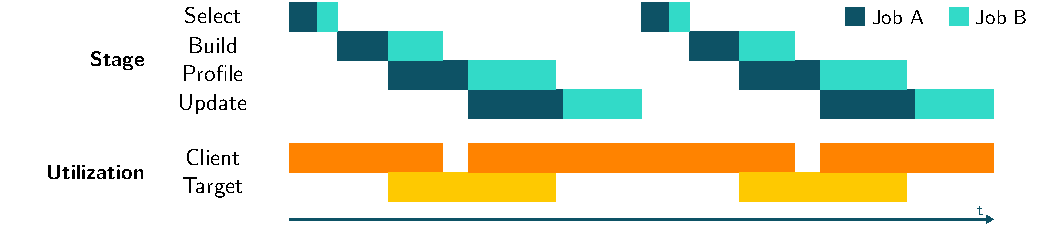
\includegraphics[width=\textwidth]{tvm_resource_utilization_interleaving}%
	\caption{Interleaved scheduler}
	\label{fig:interleaving-scheduler}
\end{figure}
Figure with autotuning procedure with scheduler
Since TVM only provides a python interface, we are using python 3.5

\subsection{RPC}
We want clients to live in different processes, docker containers, possibly physical servers (why?)
requires RPC infrastructure consisting of scheduler and clients
different from TVM RPC infrastructure
clients register to scheduler
describe endpoints

\subsection{Components}
Show whole stack, denote what happens in scheduler, what happens in runner
Show which communication is in-process and which is RPC
JobManager negotiates between autotuning stages interface and simple scheduler interface, keeps track at position in autotuning
show abstract scheduler and client interface

\subsection{Challenges}
initially wanted to run scheduler and clients in one multi-threaded process without RPC to get results quickly
not possible due to python global interpreter lock

evaluation of design choices takes long because autotuning is a slow process, created MockJob for debugging of scheduler

\section{Autotuning as a Service}
imagine autotuning as a service where users can submit their trained model and receive an optimized version according to SLA
Describe as a service
More sophisticated scheduler, requires moving more autotuning logic from client to scheduler
Make client stateless

Keep trained model and update it every n new entries to skip transfer learning time for every task
Check currently known best configurations and see if SLA is already met before actually starting autotuning
Automatically set up autotuning infrastructure
Split jobs on task and search space level to parallelize more
- make better use of unused resources
- faster autotuning, e.g. for paying customers